\chapter{Screenshots of the GUI of Gologo Application}

Following screenshots depict the graphical user interface of the application.

\begin {enumerate}
\item First time Application Users will be authenticated via PIN received through the message when NGO registers through the portal.
\begin{figure}[H]
\begin{center}   
\includegraphics[scale=0.4]{Loginscreen}
\caption{Pin Authentication}
\label{fig:pin_authenticate}
\end{center}
\end{figure}

\item Online User Registration by the NGO sends a message on registered number for authentication.
\begin{figure}[H]
\begin{center}   
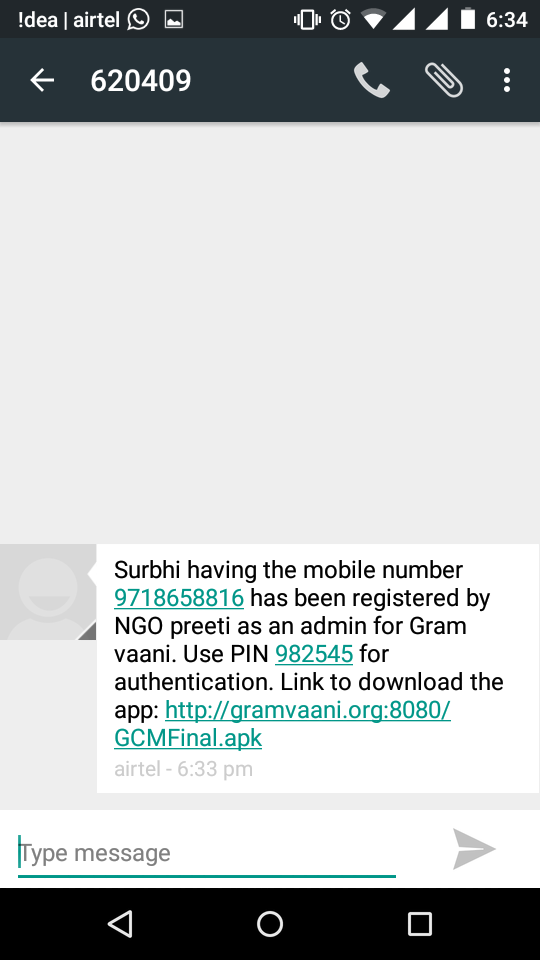
\includegraphics[scale=0.3]{authenticatemsg}
\caption{Message for Pin Authentication}
\label{fig:authenticatemsg}
\end{center}
\end{figure}

\item User can retrieve PIN by clicking on Forget PIN option.
\begin{figure}[H]
\begin{center}   
\includegraphics[scale=0.4]{Pinrecovery}
\caption{Pin Recovery}
\label{fig:pin_recovery}
\end{center}
\end{figure}

\item User will be provided with the following options.
\begin{figure}[H]
\begin{center}   
\includegraphics[scale=0.3]{Workflowapp}
\caption{Use Cases}
\label{fig:menuoptions}
\end{center}
\end{figure}

\item User can record audio by recording audio using Media Recorder.
\begin{figure}[H]
\begin{center}   
\includegraphics[scale=0.3]{Audiorecord}
\caption{Record Audio}
\label{fig:audio1}
\end{center}
\end{figure}

\item User can send instant text messages by choosing any of the below template depending upon the type of announcement.
\begin{figure}[H]
\begin{center}   
\includegraphics[scale=0.3]{Msgtemplates}
\caption{Type of Text Announcements}
\label{fig:message}
\end{center}
\end{figure}

\item Text alert of survey to be launched in the community will be sent with the specified date to inform people regarding the survey launch.
\begin{figure}[H]
\begin{center}   
\includegraphics[scale=0.4]{surveytemplate}
\caption{Announcement of Surveys}
\label{fig:message1}
\end{center}
\end{figure}

\item Text alert of upcoming camp to be organised in the community will be sent with the specified parameters to inform people. 
\begin{figure}[H]
\begin{center}   
\includegraphics[scale=0.3]{camptemplate}
\caption{Announcement of Camps(without timings)}
\label{fig:message2}
\end{center}
\end{figure}


\item  Launched scheme name along with the details of scheme date and beneficiaries for that scheme will be sent to the target people to send text alerts to inform people regarding it.
\begin{figure}[H]
\begin{center}   
\includegraphics[scale=0.3]{schemetemplate}
\caption{Announcement of Govt. Schemes}
\label{fig:message3}
\end{center}
\end{figure}

\item The app users can add a new contact. The user selects the option of Add a contact on the  home screen of application. In this option, he can fill in all the details of a new contact of his community having name, contact number, gender, date of birth, contact groups and location URI.
\begin{figure}[H]
\begin{center}   
\includegraphics[scale=0.4]{Addcontact}
\caption{Add a new contact}
\label{fig:contact1}
\end{center}
\end{figure}

\item In the above option, application user is asked for the confirmation via a diaglog box. He can either click on confirm for adding a new contact or cancel the adding of contact.
\begin{figure}[H]
\begin{center}   
\includegraphics[scale=0.4]{contactconfirm}
\caption{Add a new contact}
\label{fig:contact2}
\end{center}
\end{figure}
 
\item  Volunteers are given this functionality for the management of contact groups. Multiple contact groups are made and managed as per the groups of the community. It helps in easy dissemination of information to the relevant audience.
\begin{figure}[H]
\begin{center}   
\includegraphics[scale=0.4]{addgroup}
\caption{Add a new contact group}
\label{fig:group1}
\end{center}
\end{figure}

\item Application user can view the active survey of the GramVaani Server corresponding to the application instance.
\begin{figure}[H]
\begin{center}   
\includegraphics[scale=0.4]{launchsurvey}
\caption{List of Active Surveys}
\label{fig:viewlaunchsurvey}
\end{center}
\end{figure}

\item Application user can view a particular survey with all the survey questions along with the type of question. One can also listen the audio prompt of each survey question.
\begin{figure}[H]
\begin{center}   
\includegraphics[scale=0.3]{surveyques}
\caption{View a Particular Survey}
\label{fig:viewsurvey}
\end{center}
\end{figure}

\item  Application user can choose the target people among the gram vaani groups, his phone callers and  Mobile Vaani instance callers.
\begin{figure}[H]
\begin{center}   
\includegraphics[scale=0.4]{sendoptions}
\caption{Choose Contact Options to Launch}
\label{fig:contactoptions}
\end{center}
\end{figure}

\item Multiple Gram Vaani contact groups can be choosen as the target audience.
\begin{figure}[H]
\begin{center}   
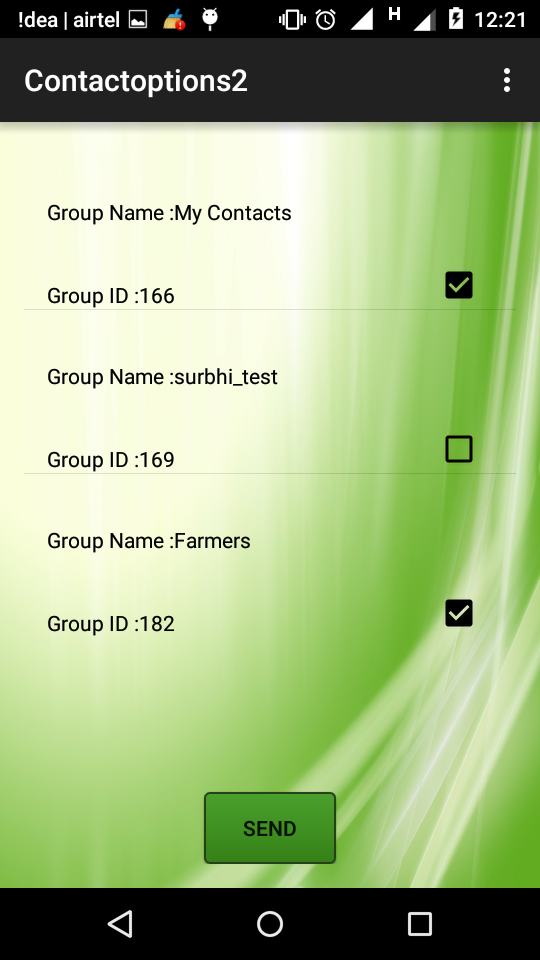
\includegraphics[scale=0.3]{contactgroups}
\caption{GV Contact Groups}
\label{fig:contactgroups}
\end{center}
\end{figure}

\item Multiple phone contacts can be choosen as the target people.
\begin{figure}[H]
\begin{center}   
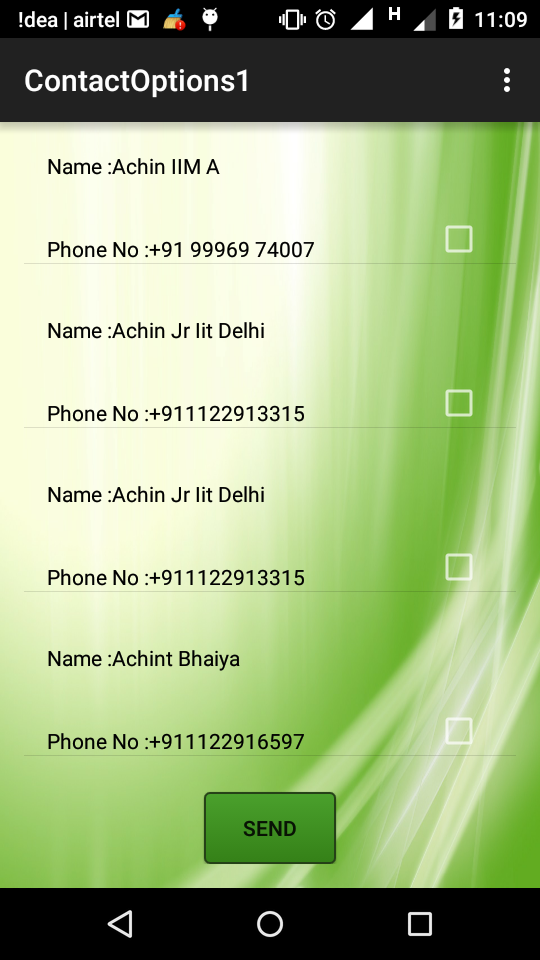
\includegraphics[scale=0.4]{phonecontacts}
\caption{Phone Contacts}
\label{fig:phonecontacts}
\end{center}
\end{figure}

\item Some quick options are provided on the application which are available across all activities. Application  user can navigate across these options.
\begin{figure}[H]
\begin{center}   
\includegraphics[width=0.8\textwidth]{Actionbaroptions}
\caption{Options on Menu Bar}
\label{fig:menubar}
\end{center}
\end{figure}

\end{enumerate}




